
\documentclass{beamer}
\usepackage[utf8]{inputenc} 	% gestion des accents (source)
\usepackage[T1]{fontenc}        % gestion des accents (PDF)
\usepackage[francais]{babel}    % gestion du français 
\usepackage{textcomp}           % caractères additionnels
\usepackage{lmodern} 			% police de caractère
\usepackage{hyperref}			% gestion des hyperliens
\hypersetup{pdfstartview=XYZ}	% Zoom par défaut

\usepackage{xcolor}			% gestion des couleurs
\usepackage{graphicx}		% gestion des images
\usepackage{wrapfig}
\usepackage{array}			%gestion améliorée des tableaux


\usepackage{subfig}
\usepackage{fancybox}
\usepackage{multicol}

\usepackage{array,multirow,makecell}
\usepackage{subfig}
\usepackage{fancybox}
\usepackage{multicol}


\usepackage{csquotes}  
% \usepackage[french]{babel} 
% \usepackage[backend=biber]{biblatex}

% Pour la coloration des fbox
\usepackage{blindtext}
\usepackage{tcolorbox}
\usepackage{graphicx}


% supporter l’UTF-8, il faut expliquer au package comment il doit se comporter quand il rencontre tel ou tel caractère. 
% Pour ce faire, on utilise l’option literate grâce à la commande lstset qui permet de préciser des options.


% Gestion des couleurs

\definecolor{monvert}{rgb}{0,0.6,0}

\definecolor{mongris}{rgb}{0.5,0.5,0.5}
\definecolor{monmauve}{rgb}{0.58,0,0.82}
\definecolor{aqua}{rgb}{0.0, 1.0, 1.0}
\definecolor{cambridgeblue}{rgb}{0.64, 0.76, 0.68}
\definecolor{orange}{rgb}{0.93, 0.57, 0.13}
\definecolor{rouge}{rgb}{1.0, 0.0, 0.22}



\definecolor{codegreen}{rgb}{0,0.6,0}
\definecolor{codegray}{rgb}{0.5,0.5,0.5}
\definecolor{codepurple}{rgb}{0.58,0,0.82}
\definecolor{backcolour}{rgb}{0.95,0.95,0.92}


% code listing settings


\usepackage{listings}
\lstset{
	language=sql,
	basicstyle=\ttfamily\small,
	aboveskip={1.0\baselineskip},
	belowskip={1.0\baselineskip},
	columns=fixed,
	extendedchars=true,
	breaklines=true,
	tabsize=4,
	prebreak=\raisebox{0ex}[0ex][0ex]{\ensuremath{\hookleftarrow}},
	frame=lines,
	showtabs=false,
	showspaces=false,
	showstringspaces=false,
	keywordstyle=\color[rgb]{0.627,0.126,0.941},
	commentstyle=\color[rgb]{0.133,0.545,0.133},
	stringstyle=\color[rgb]{01,0,0},
	%   umbers=left,
	% 	numberstyle=\small,
	%   stepnumber=1,
	%	numbersep=10pt,
	captionpos=t,
	escapeinside={\%*}{*)}
}

\lstset{
	literate=
	{á}{{\'a}}1 {é}{{\'e}}1 {í}{{\'i}}1 {ó}{{\'o}}1 {ú}{{\'u}}1
	{Á}{{\'A}}1 {É}{{\'E}}1 {Í}{{\'I}}1 {Ó}{{\'O}}1 {Ú}{{\'U}}1
	{à}{{\`a}}1 {è}{{\`e}}1 {ì}{{\`i}}1 {ò}{{\`o}}1 {ù}{{\`u}}1
	{À}{{\`A}}1 {È}{{\'E}}1 {Ì}{{\`I}}1 {Ò}{{\`O}}1 {Ù}{{\`U}}1
	{ä}{{\"a}}1 {ë}{{\"e}}1 {ï}{{\"i}}1 {ö}{{\"o}}1 {ü}{{\"u}}1
	{Ä}{{\"A}}1 {Ë}{{\"E}}1 {Ï}{{\"I}}1 {Ö}{{\"O}}1 {Ü}{{\"U}}1
	{â}{{\^a}}1 {ê}{{\^e}}1 {î}{{\^i}}1 {ô}{{\^o}}1 {û}{{\^u}}1
	{Â}{{\^A}}1 {Ê}{{\^E}}1 {Î}{{\^I}}1 {Ô}{{\^O}}1 {Û}{{\^U}}1
	{œ}{{\oe}}1 {Œ}{{\OE}}1 {æ}{{\ae}}1 {Æ}{{\AE}}1 {ß}{{\ss}}1
	{ű}{{\H{u}}}1 {Ű}{{\H{U}}}1 {ő}{{\H{o}}}1 {Ő}{{\H{O}}}1
	{ç}{{\c c}}1 {Ç}{{\c C}}1 {ø}{{\o}}1 {å}{{\r a}}1 {Å}{{\r A}}1
	{€}{{\EUR}}1 {£}{{\pounds}}1
}





% Ajout par test
 
% Ce fichier doit être éditer avec vos variables de session :
% Il est appellé dans l'ensemble de la théorie et des exercices.
% Jean-Pierre Duchesneau, hiver 2020


\newcommand{\cours}{420-W45-SF}
\newcommand{\nomcours}{Installation de serveurs et servives}
\newcommand{\session}{Hiver 2022}
\newcommand{\groupe}{???}

\newcommand{\Cegep}{Cégep Sainte-Foy, DFC}
\newcommand{\prof}{Jean-Pierre Duchesneau}
\newcommand{\initiales}{JPD}


\newcommand{\Auteur}{Jean-Pierre Duchesneau} % apparait à la fin dans les droits d'auteurs
\newcommand{\dateRedaction}{Hiver 2022}

\newcommand{\SELinux}{Ubuntu 20.04 LTS }
\newcommand{\SEWin}{Windows 10 20H2}

\newcommand{\Esx}{VMware vSphere : \url{https://vcenterdfc.csfoy.ca}}
\newcommand{\VmRep}{H22\_S4\_4392\_GEN}
\newcommand{\version}{1.0.1}


\newcommand{\projetgit}{introGit}

\newcommand{\srvGit}{https://github.com/jpduchesneauCegep/}

\newcommand{\srvGitProjet}{https://github.com/jpduchesneauCegep/IntroGit.git}
%\usetheme{Marburg} % Menu à droite
%\usetheme{Boadilla} % Sans menu bleu
\usetheme{CambridgeUS}  %Sans menu rouge

% ======================================================
% Debut - Rédaction du diaporama

\begin{document}
	
	\title[Intro Internet]{ Cours 1 -
		Introduction aux services Internet}
	\author[\initiales]{\prof \\ DFC - Cégep de Sainte-Foy}
	\institute{\nomcours\\ \cours}
	
	
	\date{\null}
	% ======================================================
	% Début diapo
	
	\begin{frame}
		\titlepage
	\end{frame}
	
	
	
	% ======================================================
	
	% Diapo 3 Retour sur les cours précédents ==============================================================
	
	\section{Thèmes}
	
	\begin{frame}[containsverbatim]
		
		\frametitle{Thèmes}
		
		\begin{itemize}
			\item Présentation de plan de cours
			\item Place du cours dans le programme
			
			\item Répertorier les principaux services de l’Internet
			\item Architecture réseau
			\item Stockage
		\end{itemize}
	\end{frame}
	\section{Les services de l’Internet}
	\begin{frame}
		\frametitle{Mettre en opération des services de
			communication utilisés dans l’Internet/Intranet}
		
		\begin{itemize}
			\item  Un réseau c'est quoi ?
			\item La différence entre des services et
			des applications?
			\item Internet qu'est-ce?
			\begin{itemize}
				\item Protocole IP
				\item Quelles applications?
			\end{itemize}
			
			\item La différence entre les deux ?
			\item Pourquoi appelle-t-on Internet le réseau des
			réseaux
			?\end{itemize}
	\end{frame}
	\begin{frame}[containsverbatim]
		\frametitle{Histoire des services de l'Internet}
		\begin{itemize}
			\item  En 1972, la première application importante : le
			courrier électronique.
			\item 1979 Usenet, qui deviendra en 2005 Google Groups
			\item 1980, le FTP
			\item 1983, DNS et avant?
			\item Le début des années 1990 marque, en fait, la
			naissance d'Internet tel que nous le connaissons
			aujourd'hui : le Web, un ensemble de pages en
			HTML mélangeant du texte, des liens, des images,
			adressables via une URL et accessibles via le
			protocole HTTP.
			\item  Pour l'historique plus complet d'Internet, voir :
			\url{ http://fr.wikipedia.org/wiki/Internet}
		\end{itemize}
		
	\end{frame}
	
	
	\begin{frame}[containsverbatim]
		\frametitle{Applications de l’Internet}
		\begin{itemize}
			\item Utilisées dans un réseau fermé;
			\item Utilisées dans un réseau local relié à l’Internet;
			\item Utilisées entre deux réseaux locaux reliés en Réseau privé virtuel (infonuagique);
			\item Utilisées sous de multiples combinaisons.
			
		\end{itemize}
		
	\end{frame}
	
	\begin{frame}[containsverbatim]
		\frametitle{Applications – clients / serveurs }
		\begin{itemize}
			\item  Serveur(s) de fichiers, NAS, SAN (pour le partage des données)
			\item Serveur de base de données (pour le stockage des informations)
			\item Serveur WEB
			\item Serveur FTP pour le transfert des fichiers
			
			\item Serveur de courrier – Clients SMTP, POP et IMAP
			\item Serveur de communication sécurisée – SSH
			\item Serveur(s) d'authentification (pour l'identification des utilisateurs et le
			stockage des annuaires, protocole LDAP)
			\item Serveur spécialisé – client spécialisé.
			\item Serveur(s) et logiciel client de supervision réseau/systèmes (le protocole SNMP)
			\item Serveur de contrôle distant 
		\end{itemize}
		
		
	\end{frame}
	\section{Réseau}
	
	\begin{frame}[containsverbatim]
		\frametitle{Où sont situés les services}
		\begin{itemize}
			\item Dans les réseaux locaux et les WAN.
			\item Dans Internet ?
			\item Dans la DMZ
		\end{itemize}
		
	\end{frame}
	\begin{frame}[containsverbatim]
		\frametitle{DMZ (Zone démilitarisée)}
		\begin{itemize}
			\item  Un sous-réseau séparé du réseau local et isolé de celui-ci et
			d'Internet par un pare-feu.
			\item Ce sous-réseau contient les machines étant susceptibles d'être
			accédées depuis Internet.
			\item Le pare-feu bloquera donc les accès au réseau local pour
			garantir sa sécurité.
		\end{itemize}
		\begin{figure}[!h]
			\centering
			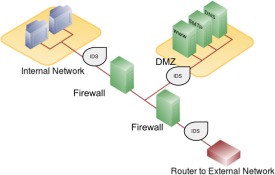
\includegraphics[scale=0.6]{images/dmz}
			\caption{DMZ}
			\label{rand}
		\end{figure}
		
		
	\end{frame}
	\section{Stockage}
	\begin{frame}[containsverbatim]
		\frametitle{ET le stockage}
		Type : 
		\begin{itemize}
			\item  \textbf{DAS} : Direct Attached Storage, c'est-à-dire un disque dur
			directement connecté à l'ordinateur qui utilise les protocoles
			ATA, SATA, eSATA, SCSI, SAS et Fibre Channel via des
			câbles dédiés.
			\item \textbf{NAS}: Network Attached Storage, fournit des services à
			travers un réseau IP avec un ou plusieurs des protocoles
			suivants : SMB(CIFS), NFS, AFP.
			\item \textbf{SAN} : Storage Area Network (SAN) qui utilise les protocoles
			comme SCSI, Fibre Channel, iSCSI, ATA over Ethernet
			(AoE) ou HyperSCSI  à travers un réseau dédié ;
		\end{itemize}
		
		
	\end{frame}
	
	
	\begin{frame}[containsverbatim]
		\frametitle{Exemple de stockage : Nos serveurs}
		\begin{figure}[!h]
			\centering
			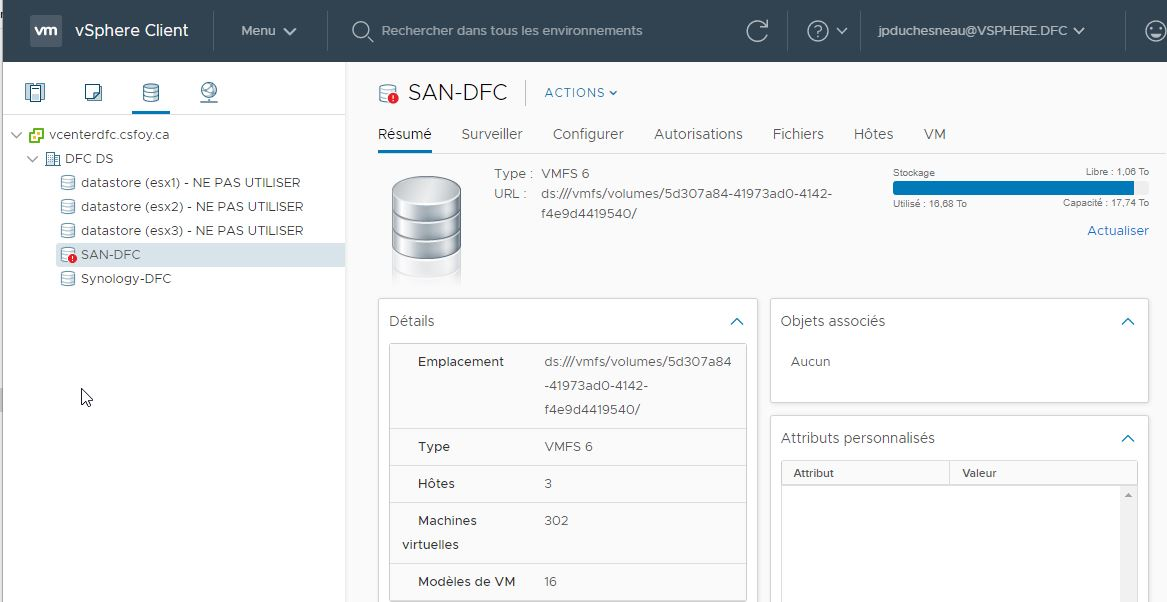
\includegraphics[scale=0.4]{images/SAN}
			\caption{SAN de l'infrastructure vSphere}
			\label{rand}
		\end{figure}
		
	\end{frame}
	
	
	
	\begin{frame}[containsverbatim]
		\frametitle{Schéma d'un SAN}
		\begin{figure}
			\centering
			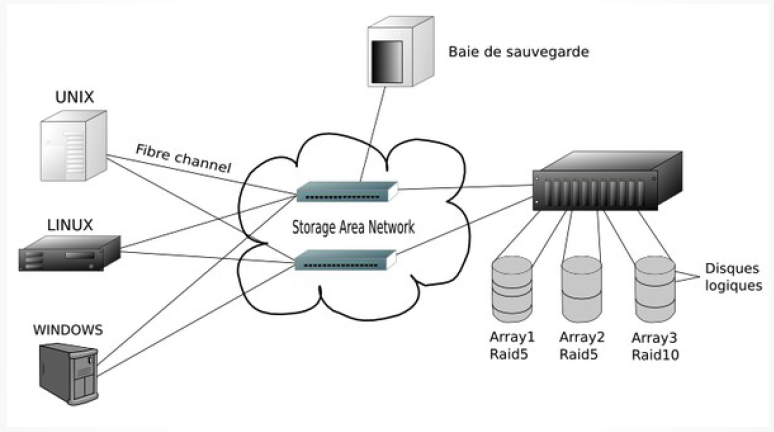
\includegraphics[scale=0.6]{images/image1}
		\end{figure}
		
		
	\end{frame}
	
	
	\begin{frame}[containsverbatim]
		\frametitle{RAID} 
		{\small Le RAID (Redundant Array of Independent Disks)  permet de répartir des données sur plusieurs disques durs afin d'améliorer soit les performances, soit la sécurité ou la tolérance aux pannes de l'ensemble du ou des systèmes.
			
			Le système RAID est :
			\begin{itemize}
				\item   soit un système de redondance qui donne au stockage des données une certaine tolérance aux pannes matérielles (ex. : RAID 1).
				\item soit un système de répartition qui améliore ses performances (ex. : RAID 0).
				\item soit les deux à la fois, mais avec une moins bonne efficacité (ex. : RAID 5).
			\end{itemize}
			
			
			
			Le système RAID est donc capable de gérer d'une manière ou d'une autre la répartition et la cohérence de ces données. Ce système de contrôle peut être purement logiciel ou utiliser un matériel dédié.}
		
		{\tiny {\footnotesize Source : \url{https://fr.wikipedia.org/wiki/RAID_(informatique)}}}
	\end{frame}
	
	
	
	\subsection{Logical Volume Manager}
	\begin{frame}
		\frametitle{Logical Volume Manager}
		Le gestionnaire de volumes logiques permet la création et la gestion de volumes logique sous Linux. L'utilisation de volumes logiques remplace en quelque sorte le partitionnement des disques.\\
		
		C'est un système beaucoup plus souple, qui permet par exemple de diminuer la taille d'un système de fichier pour pouvoir en agrandir un autre, sans se préoccuper de leur emplacement sur le disque.\\
		\vspace{10pt}
		\fcolorbox{black}{orange}{
			\begin{minipage}{11cm}
				\textbf{C'est essentiel dans la majorité des serveurs de données ou des serveurs de bases de données sur site (on-premise).}
		\end{minipage}}
		
		
	\end{frame}
	\begin{frame}[containsverbatim]
		\frametitle{LVM }
		\begin{figure}[!h]
			\centering
			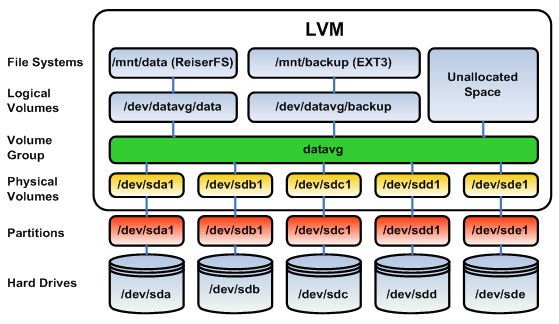
\includegraphics[scale=0.5]{images/Lvm1}
		\end{figure}
	\end{frame}
	
	\subsection{Système de fichier réseau}
	
	\begin{frame}[containsverbatim]
		\frametitle{Système de fichier réseau}
		\begin{itemize}
			\item  NFS (Network File System) : tous les UNIX, Linux, Mac OS X, IRIX et Windows pour la version 4.
			\item SMB (Server Message Block) : est un protocole permettant le partage de ressources (fichiers et imprimantes) sur des réseaux locaux avec des PC sous Windows. Il a également été appelé CIFS dans NT4. 
			Actuellement version 3.1.1 sur Windows 10 et Windows Server 2016.
			\item SAMBA : Le protocole SMB est disponible sur la plupart des systèmes d'exploitation, notamment Linux/Unix, grâce à son implémentation libre Samba.
			
		\end{itemize}
		
	\end{frame}
	
	
	% =======================================================================================================
	% Fin la suite :
	\section{À faire}
	
	\begin{frame}
		\frametitle{À faire}
		
		
		\textbf{Exercice} 
		\begin{itemize}
			\item Installation de votre machine virtuelle\\
			
		\end{itemize}
		\textbf{Écoute pour le prochain cours} 
		\begin{itemize}
			\item \href{https://binged.it/3Mi3RVE}{Fonctionnement DNS : https://binged.it/3Mi3RVE}
			\begin{itemize}
				\item Partie 1 : Les principes généraux, DNS et DHCP dans un réseau local(14 minutes)
				\item parti 2 : Le fonctionnement d'un service DNS. Composition des noms de domaines. (de 14 à 23 minutes)
				\item Partie 3 : Les enregistrements et leurs rôles. (de 23 minutes à 29 minutes)
				\item Partie 4 : La notion de serveur d'autorité versus cache. (de 29 minutes à 35 minutes)
				\item Partie 5 : Reverse DNS (de 35 à 43 minutes)
			\end{itemize}
			
			
		\end{itemize}
		
		
	\end{frame}
	
\end{document}
% Fin - Rédaction du diaporama

